\documentclass{standalone}
\usepackage{tikz}
\usetikzlibrary{patterns, positioning}


\begin{document}
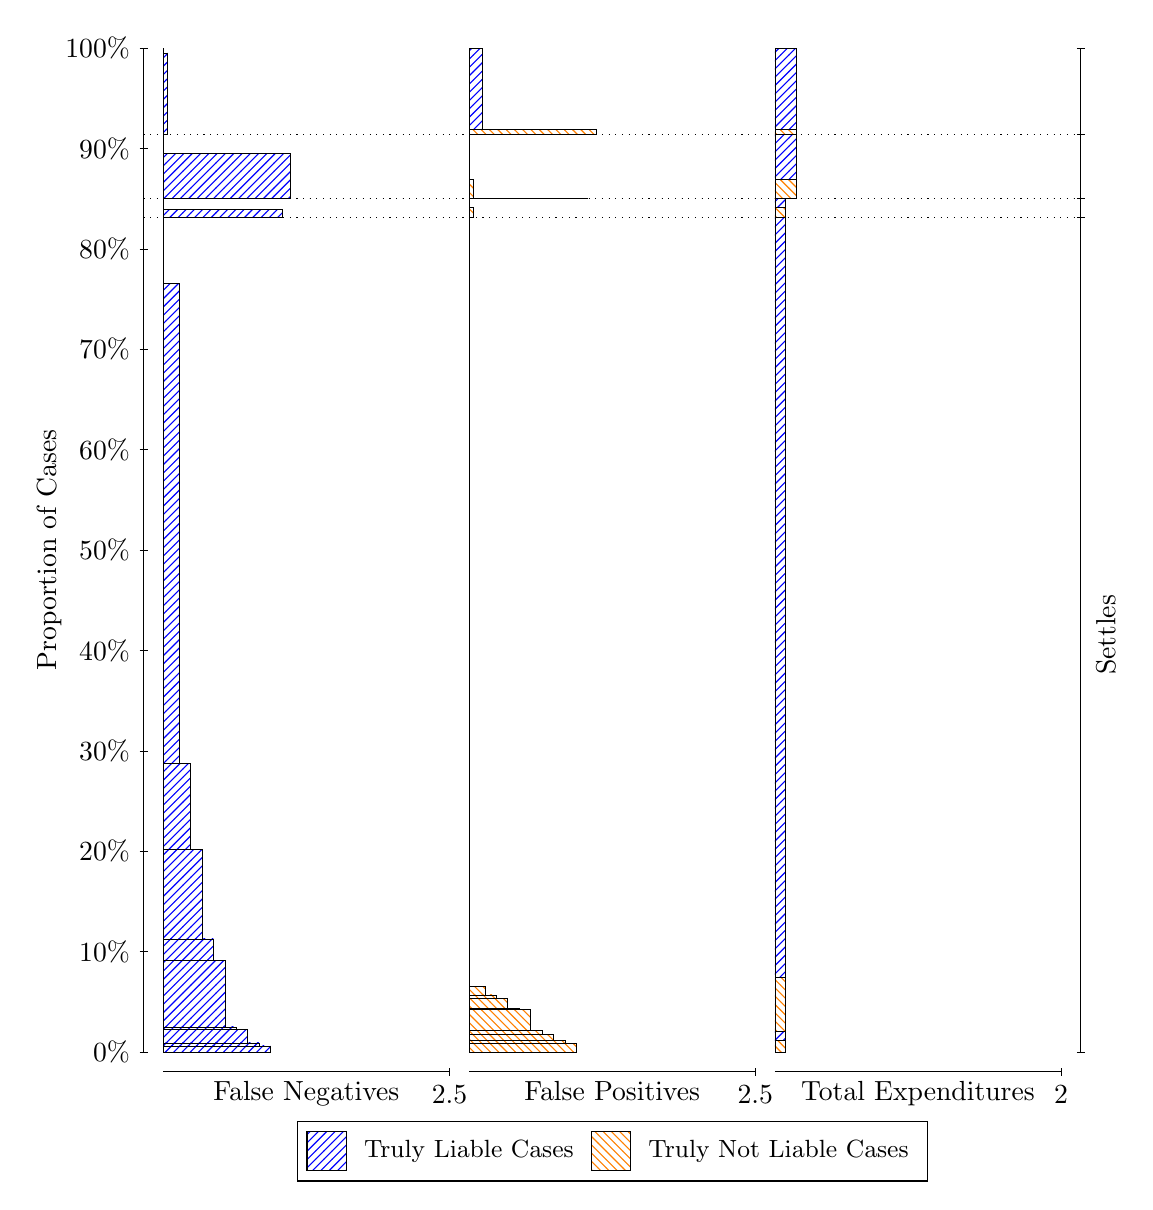
\begin{tikzpicture}
\draw[black, very thin] (1.5,1.75) -- (1.5,14.5);
\node[rotate=90, text=black, anchor=center] at (0.3, 8.125) {Proportion of Cases};
\draw[black, very thin] (1.45,1.75) -- (1.55,1.75);
\node[text=black, anchor=east] at (1.45, 1.75) {0\%};
\draw[black, very thin] (1.45,3.025) -- (1.55,3.025);
\node[text=black, anchor=east] at (1.45, 3.025) {10\%};
\draw[black, very thin] (1.45,4.3) -- (1.55,4.3);
\node[text=black, anchor=east] at (1.45, 4.3) {20\%};
\draw[black, very thin] (1.45,5.575) -- (1.55,5.575);
\node[text=black, anchor=east] at (1.45, 5.575) {30\%};
\draw[black, very thin] (1.45,6.85) -- (1.55,6.85);
\node[text=black, anchor=east] at (1.45, 6.85) {40\%};
\draw[black, very thin] (1.45,8.125) -- (1.55,8.125);
\node[text=black, anchor=east] at (1.45, 8.125) {50\%};
\draw[black, very thin] (1.45,9.4) -- (1.55,9.4);
\node[text=black, anchor=east] at (1.45, 9.4) {60\%};
\draw[black, very thin] (1.45,10.675) -- (1.55,10.675);
\node[text=black, anchor=east] at (1.45, 10.675) {70\%};
\draw[black, very thin] (1.45,11.95) -- (1.55,11.95);
\node[text=black, anchor=east] at (1.45, 11.95) {80\%};
\draw[black, very thin] (1.45,13.225) -- (1.55,13.225);
\node[text=black, anchor=east] at (1.45, 13.225) {90\%};
\draw[black, very thin] (1.45,14.5) -- (1.55,14.5);
\node[text=black, anchor=east] at (1.45, 14.5) {100\%};

\draw[black, very thin] (13.4,1.75) -- (13.4,14.5);
\draw[black, very thin] (13.35,1.75) -- (13.45,1.75);
\node[anchor=west] at (13.35, 1.75) {};
\draw[black, very thin] (13.35,12.345) -- (13.45,12.345);
\node[anchor=west] at (13.35, 12.345) {};
\draw[black, very thin] (13.35,12.586) -- (13.45,12.586);
\node[anchor=west] at (13.35, 12.586) {};
\draw[black, very thin] (13.35,12.594) -- (13.45,12.594);
\node[anchor=west] at (13.35, 12.594) {};
\draw[black, very thin] (13.35,13.405) -- (13.45,13.405);
\node[anchor=west] at (13.35, 13.405) {};
\draw[black, very thin] (13.35,14.5) -- (13.45,14.5);
\node[anchor=west] at (13.35, 14.5) {};

\draw[black, very thin, pattern color=blue, pattern=north east lines] (1.75,1.75) rectangle (3.1125,1.8276);
\draw[black, very thin, pattern color=blue, pattern=north east lines] (1.75,1.8276) rectangle (2.9672,1.8656);
\draw[black, very thin, pattern color=blue, pattern=north east lines] (1.75,1.8656) rectangle (2.8218,2.0372);
\draw[black, very thin, pattern color=blue, pattern=north east lines] (1.75,2.0372) rectangle (2.6765,2.069);
\draw[black, very thin, pattern color=blue, pattern=north east lines] (1.75,2.069) rectangle (2.5312,2.9094);
\draw[black, very thin, pattern color=blue, pattern=north east lines] (1.75,2.9094) rectangle (2.3858,3.1854);
\draw[black, very thin, pattern color=blue, pattern=north east lines] (1.75,3.1854) rectangle (2.2405,4.3202);
\draw[black, very thin, pattern color=blue, pattern=north east lines] (1.75,4.3202) rectangle (2.0952,5.4122);
\draw[black, very thin, pattern color=blue, pattern=north east lines] (1.75,5.4122) rectangle (1.9498,11.509);
\draw[black, very thin, pattern color=orange, pattern=north west lines] (1.75,11.509) rectangle (1.75,12.345);
\draw[black, very thin, pattern color=blue, pattern=north east lines] (1.75,12.345) rectangle (3.2578,12.45);
\draw[black, very thin, pattern color=orange, pattern=north west lines] (1.75,12.45) rectangle (1.75,12.586);
\draw[black, very thin, pattern color=blue, pattern=north east lines] (1.75,12.586) rectangle (1.8045,12.593);
\draw[black, very thin, pattern color=orange, pattern=north west lines] (1.75,12.593) rectangle (1.75,12.594);
\draw[black, very thin, pattern color=blue, pattern=north east lines] (1.75,12.594) rectangle (3.3668,13.165);
\draw[black, very thin, pattern color=orange, pattern=north west lines] (1.75,13.165) rectangle (1.75,13.405);
\draw[black, very thin, pattern color=blue, pattern=north east lines] (1.75,13.405) rectangle (1.8045,14.437);
\draw[black, very thin, pattern color=orange, pattern=north west lines] (1.75,14.437) rectangle (1.75,14.5);
\draw[black, very thin, pattern color=orange, pattern=north west lines] (5.6333,1.75) rectangle (6.9958,1.8637);
\draw[black, very thin, pattern color=orange, pattern=north west lines] (5.6333,1.8637) rectangle (6.8505,1.8945);
\draw[black, very thin, pattern color=orange, pattern=north west lines] (5.6333,1.8945) rectangle (6.7052,1.9767);
\draw[black, very thin, pattern color=orange, pattern=north west lines] (5.6333,1.9767) rectangle (6.5598,2.0248);
\draw[black, very thin, pattern color=orange, pattern=north west lines] (5.6333,2.0248) rectangle (6.4145,2.2875);
\draw[black, very thin, pattern color=orange, pattern=north west lines] (5.6333,2.2875) rectangle (6.2692,2.3044);
\draw[black, very thin, pattern color=orange, pattern=north west lines] (5.6333,2.3044) rectangle (6.1238,2.4355);
\draw[black, very thin, pattern color=orange, pattern=north west lines] (5.6333,2.4355) rectangle (5.9785,2.4746);
\draw[black, very thin, pattern color=orange, pattern=north west lines] (5.6333,2.4746) rectangle (5.8332,2.5859);
\draw[black, very thin, pattern color=blue, pattern=north east lines] (5.6333,2.5859) rectangle (5.6333,12.345);
\draw[black, very thin, pattern color=orange, pattern=north west lines] (5.6333,12.345) rectangle (5.6878,12.481);
\draw[black, very thin, pattern color=blue, pattern=north east lines] (5.6333,12.481) rectangle (5.6333,12.586);
\draw[black, very thin, pattern color=orange, pattern=north west lines] (5.6333,12.586) rectangle (7.1412,12.586);
\draw[black, very thin, pattern color=blue, pattern=north east lines] (5.6333,12.586) rectangle (5.6878,12.594);
\draw[black, very thin, pattern color=orange, pattern=north west lines] (5.6333,12.594) rectangle (5.6878,12.834);
\draw[black, very thin, pattern color=blue, pattern=north east lines] (5.6333,12.834) rectangle (5.6333,13.405);
\draw[black, very thin, pattern color=orange, pattern=north west lines] (5.6333,13.405) rectangle (7.2502,13.468);
\draw[black, very thin, pattern color=blue, pattern=north east lines] (5.6333,13.468) rectangle (5.7968,14.5);
\draw[black, very thin, pattern color=orange, pattern=north west lines] (9.5167,1.75) rectangle (9.6529,1.9004);
\draw[black, very thin, pattern color=blue, pattern=north east lines] (9.5167,1.9004) rectangle (9.6529,2.016);
\draw[black, very thin, pattern color=orange, pattern=north west lines] (9.5167,2.016) rectangle (9.6529,2.7015);
\draw[black, very thin, pattern color=blue, pattern=north east lines] (9.5167,2.7015) rectangle (9.6529,12.345);
\draw[black, very thin, pattern color=orange, pattern=north west lines] (9.5167,12.345) rectangle (9.6529,12.481);
\draw[black, very thin, pattern color=blue, pattern=north east lines] (9.5167,12.481) rectangle (9.6529,12.586);
\draw[black, very thin, pattern color=orange, pattern=north west lines] (9.5167,12.586) rectangle (9.6529,12.586);
\draw[black, very thin, pattern color=blue, pattern=north east lines] (9.5167,12.586) rectangle (9.6529,12.594);
\draw[black, very thin, pattern color=orange, pattern=north west lines] (9.5167,12.594) rectangle (9.7892,12.834);
\draw[black, very thin, pattern color=blue, pattern=north east lines] (9.5167,12.834) rectangle (9.7892,13.405);
\draw[black, very thin, pattern color=orange, pattern=north west lines] (9.5167,13.405) rectangle (9.7892,13.468);
\draw[black, very thin, pattern color=blue, pattern=north east lines] (9.5167,13.468) rectangle (9.7892,14.5);
\draw[black, dotted] (1.5,12.345) -- (13.4,12.345);
\draw[black, dotted] (1.5,12.586) -- (13.4,12.586);
\draw[black, dotted] (1.5,12.594) -- (13.4,12.594);
\draw[black, dotted] (1.5,13.405) -- (13.4,13.405);
\draw[black, very thin] (1.75,1.5) -- (5.3833,1.5);
\node[text=black, anchor=north] at (3.5667, 1.5) {False Negatives};
\draw[black, very thin] (5.3833,1.45) -- (5.3833,1.55);
\node[text=black, anchor=north] at (5.3833, 1.45) {2.5};

\draw[black, very thin] (5.6333,1.5) -- (9.2667,1.5);
\node[text=black, anchor=north] at (7.45, 1.5) {False Positives};
\draw[black, very thin] (9.2667,1.45) -- (9.2667,1.55);
\node[text=black, anchor=north] at (9.2667, 1.45) {2.5};

\draw[black, very thin] (9.5167,1.5) -- (13.15,1.5);
\node[text=black, anchor=north] at (11.333, 1.5) {Total Expenditures};
\draw[black, very thin] (13.15,1.45) -- (13.15,1.55);
\node[text=black, anchor=north] at (13.15, 1.45) {2};

\node[text=black, centered, rotate=90] at (13.72, 7.0474) {Settles};





\draw (7.449999999999999,1.5) node[draw=none] (baseCoordinate) {};
\begin{scope}[align=center]
        \matrix[scale=0.5, draw=black, below=0.5cm of baseCoordinate, nodes={draw}, column sep=0.1cm]{
            \node[rectangle, draw, minimum width=0.5cm, minimum height=0.5cm, pattern color=blue, pattern=north east lines] {}; &
            \node[draw=none, font=\small, text=black] (B) {Truly Liable Cases}; &
            \node[rectangle, draw, minimum width=0.5cm, minimum height=0.5cm, pattern color=orange, pattern=north west lines] {}; &
            \node[draw=none, font=\small, text=black] (B) {Truly Not Liable Cases}; \\
            };
\end{scope}

\end{tikzpicture}
\end{document}